\subsection{Hough Transform}

Vi bruger Hough transformationen til at finde linjerne i billedet. For at kunne gøre dette skal vi have et BW billede. Ligning~\ref{eq:hough} viser udtrykket, hvor $\theta$ er vinkelen til x-aksen og $\rho$ er den vinkelrette afstand til origo.

\begin{equation}\label{eq:hough}
x \; cos(\theta) + y \; sin(\theta) = \rho
\end{equation}

\begin{figure}[H]
	\centering
	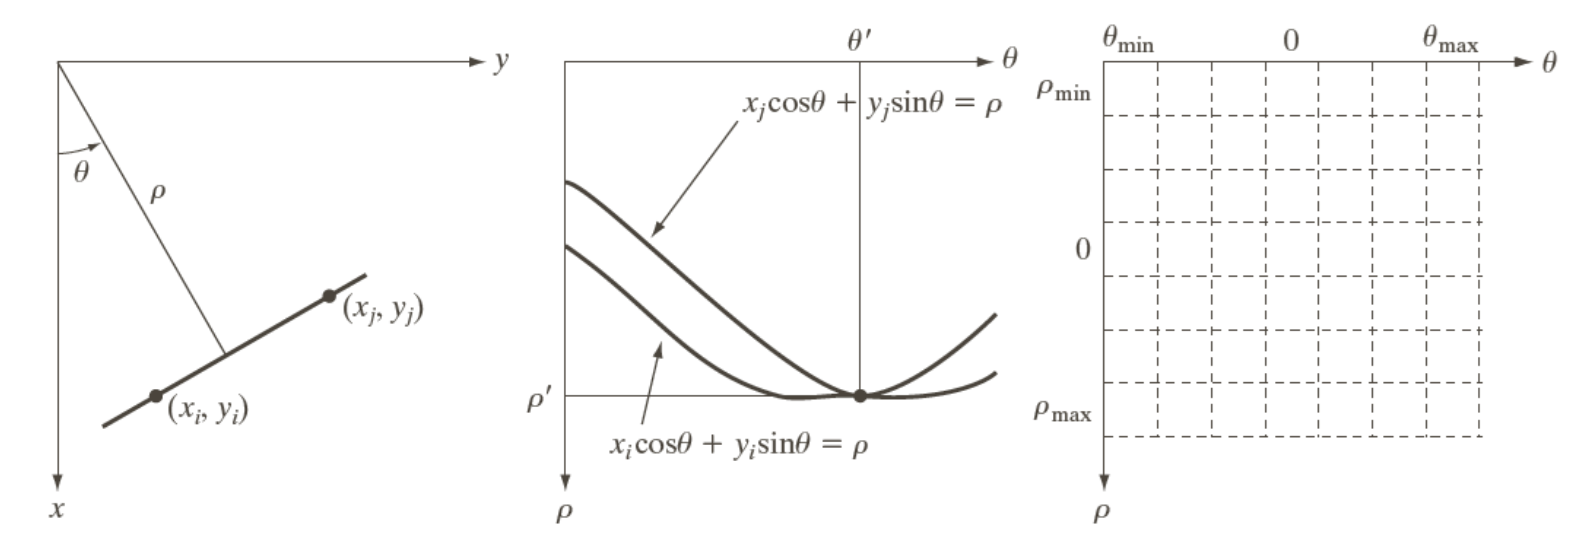
\includegraphics[width=0.9\linewidth]{figs/spm11/hough-transform-graph}
	\caption{Illustration af Hough transformationen.}
	\label{fig:hough-transform-graph}
\end{figure}

Figur~\ref{fig:hough-airport} viser et anvend eksempel på Hough transformationen. I normal læseretning viser billederne: 

\begin{figure}[H]
	\centering
	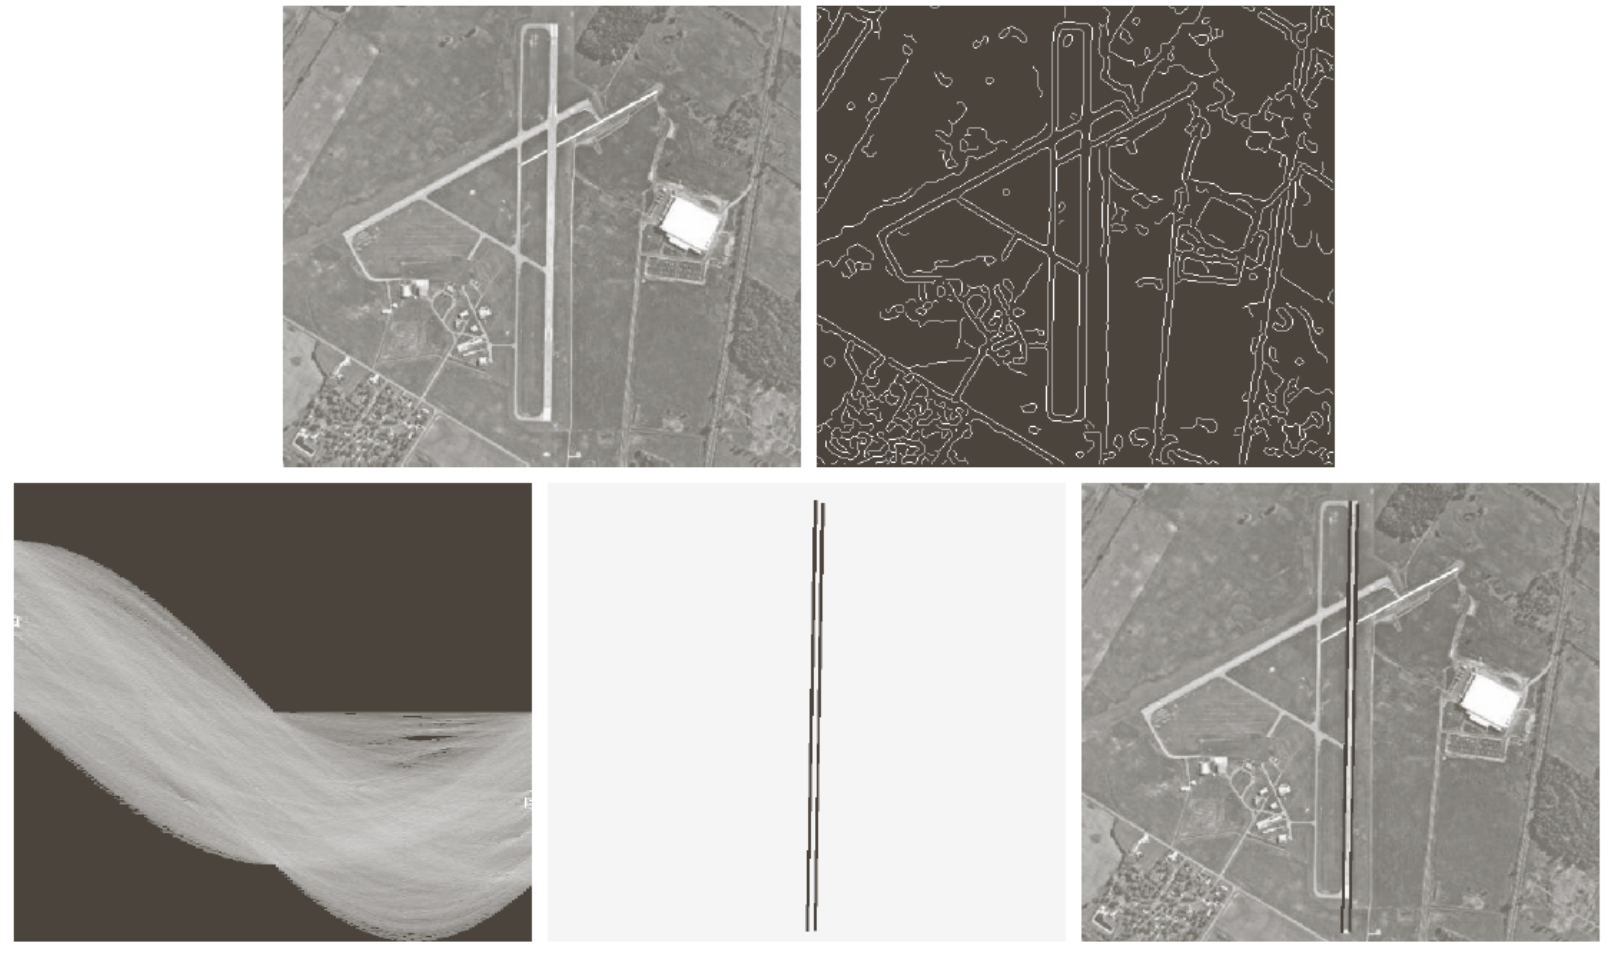
\includegraphics[width=\linewidth]{figs/spm11/hough-airport}
	\caption{Eksempel på anvendelse af Hough.}
	\label{fig:hough-airport}
\end{figure}

\vbox{%
\begin{enumerate}
	\item Det originale billede.
	\item Kantbillede efter Canny algoritmen.
	\item Hough paramenter space.
	\item Linjerne i billedet som parameter space'et fandt.
	\item Lines superimposed on the original.
\end{enumerate}}

\begin{figure}[H]
	\centering
	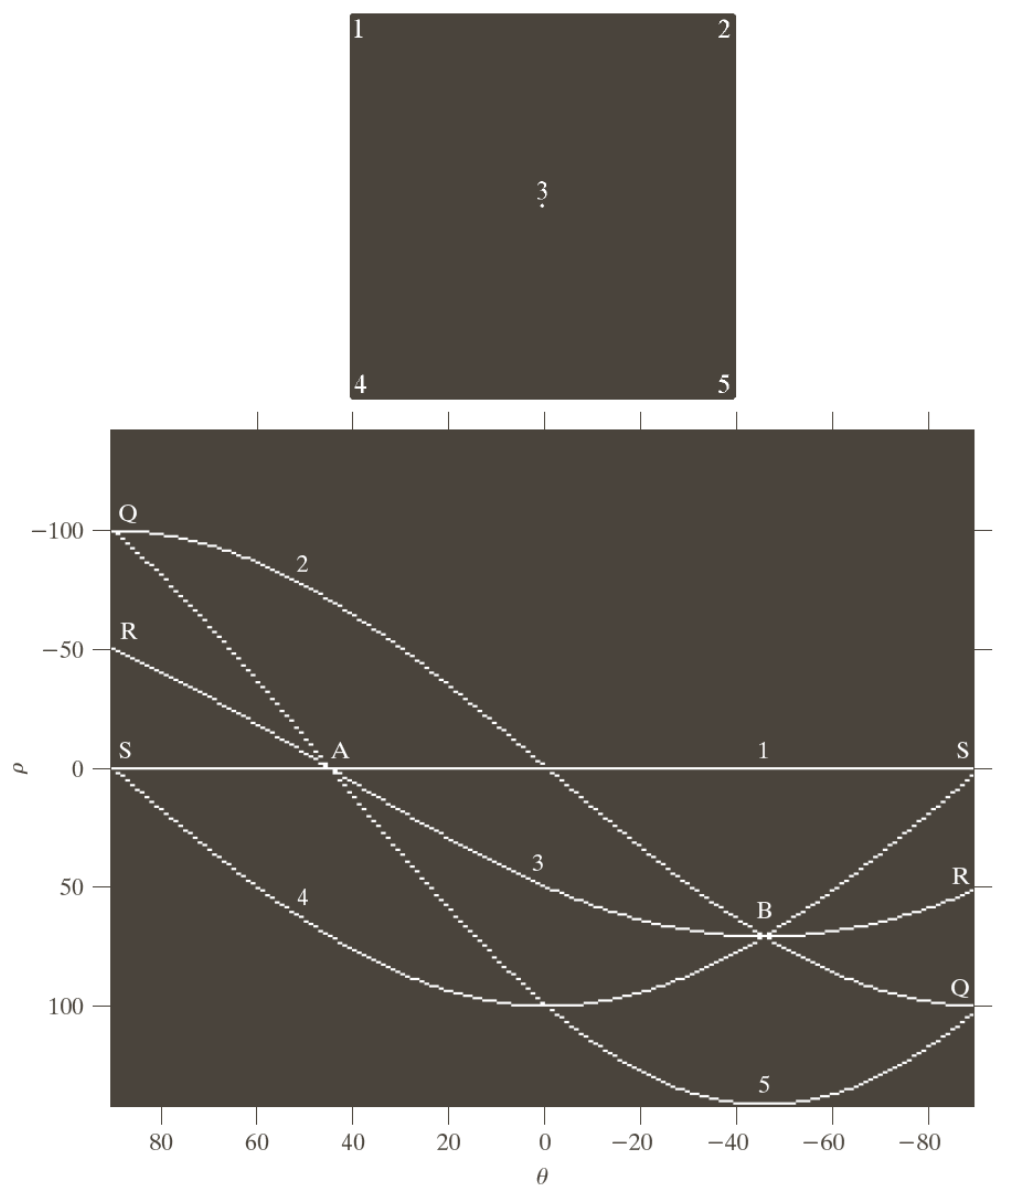
\includegraphics[width=0.7\linewidth]{figs/spm11/hough-bw}
	\caption{Argumentbeskrivelse af Hough.}
	\label{fig:hough-bw}
\end{figure}

Figur~\ref{fig:hough-bw} skal bruges til hurtigt at forklare Hough parameter space i forhold til punkter i et billede.
